\documentclass[journal]{IEEEtran}

\usepackage{cite}
\usepackage{amsmath,amssymb,amsfonts}
\usepackage{graphicx}
\usepackage{textcomp}
\usepackage{xcolor}
\usepackage{booktabs}
\usepackage{url}
\graphicspath{{figs/}}

\def\BibTeX{{\rm B\kern-.05em{\sc i\kern-.025em b}\kern-.08em
    T\kern-.1667em\lower.7ex\hbox{E}\kern-.125emX}}

\begin{document}

\title{Dynamic-Envelope Re-Tuning of a Graph-Theoretic Swarm
Formation Planner for School-Like Robotic-Fish Behavior:\\
A Controlled Simulation Study}

\author{Chinmay~Kulkarni% <-this % stops a space
\thanks{Manuscript prepared June~2026.}%
\thanks{The author is with the Robotic-Fish Swarm Project. Source code,
data, and figures are available at the project repository.}%
\thanks{This work builds on the open-source ZJU-FAST-Lab
\emph{Swarm-Formation} framework~\cite{quan2022distributed}.}}

\markboth{Manuscript -- Robotic-Fish Swarm Formation}%
{Kulkarni: Dynamic-Envelope Re-Tuning of a Graph-Theoretic Swarm Formation Planner}

\maketitle

\begin{abstract}
Distributed trajectory optimizers can fly a rigid swarm formation through
cluttered space, but the motion they produce is shaped as much by the
\emph{dynamic-feasibility envelope}---the velocity and acceleration limits
fed to the optimizer---as by the planner itself. Biological schools of fish
move slowly and smoothly, with drag-limited accelerations, in marked
contrast to the aggressive, jerk-rich trajectories typical of quadrotor
swarms. We ask a focused, reproducible question: holding a state-of-the-art
graph-theoretic formation planner and the obstacle field fixed, how does
contracting the dynamic envelope from quadrotor values to fish-like values
change the swarm's kinematics, timing, formation accuracy, and safety? We
re-skin the agents of an open-source seven-robot formation planner as a
school of robotic fish and re-tune only their motion envelope
($v_{\max}\!:\!1.5\!\rightarrow\!1.0~\mathrm{m/s}$,
$a_{\max}\!:\!8.0\!\rightarrow\!2.5~\mathrm{m/s^2}$), then run a controlled
headless study across five obstacle seeds per condition. The fish envelope
roughly \emph{halves} root-mean-square (RMS) jerk ($0.66\!\rightarrow\!0.34~\mathrm{m/s^3}$)
and cuts mean acceleration by $\sim$44\%, producing visibly smoother,
lower-effort motion, at the cost of $\sim$44\% longer traversal time. Crucially,
formation accuracy, inter-agent spacing, obstacle clearance, and a 100\%
mission-success rate are all preserved within run-to-run noise. The results
quantify a clean time-versus-smoothness trade-off and show that a
graph-theoretic formation planner degrades gracefully under a strongly
contracted, bio-inspired dynamic envelope.
\end{abstract}

\begin{IEEEkeywords}
Swarm robotics, formation control, trajectory optimization, bio-inspired
robotics, robotic fish, multi-robot systems.
\end{IEEEkeywords}

\IEEEpeerreviewmaketitle

\section{Introduction}
\IEEEPARstart{C}{oordinated} motion of a multi-robot team in a rigid,
shape-preserving formation is a core capability for aerial inspection,
collective transport, cooperative mapping, and underwater monitoring. The
hard version of the problem couples three requirements that pull against
one another: each robot must (i) hold its place in a desired geometric
\emph{formation}, (ii) avoid static obstacles and its neighbors, and
(iii) respect its own \emph{dynamic limits}. Recent distributed
spatio-temporal optimizers solve all three jointly and in real time. In
particular, the \emph{Swarm-Formation} framework of Quan
\emph{et~al.}~\cite{quan2022distributed,quan2023robust} introduces a
differentiable, graph-theoretic measure of formation similarity and folds
it into a per-agent trajectory optimizer built on the
EGO-Swarm~\cite{zhou2021egoswarm} and MINCO~\cite{wang2022geometrically}
machinery, enabling a swarm of quadrotors to weave through a dense forest
while holding shape.

A property that is easy to overlook is that the \emph{shape} of the executed
motion---how fast, how aggressively, how smoothly the swarm moves---is
governed not only by the planner but by the \emph{dynamic-feasibility
envelope}, i.e.\ the maximum velocity $v_{\max}$ and acceleration $a_{\max}$
the optimizer is told to respect. Quadrotors are typically given a large
envelope and consequently fly fast, jerky trajectories. Biological systems
at the other extreme---a school of fish~\cite{katz2011inferring}, a flock of
birds~\cite{reynolds1987flocks}---move comparatively slowly and smoothly,
their accelerations bounded by hydrodynamic or aerodynamic drag. This
contrast motivates a concrete question with direct engineering relevance for
slow, drag-limited platforms such as underwater
vehicles~\cite{berlinger2021implicit,scharff2018sensing}:

\begin{quote}
\emph{If we keep a state-of-the-art formation planner and the environment
fixed and only contract the dynamic envelope from quadrotor values to
fish-like values, what exactly do we gain and what do we lose?}
\end{quote}

This paper answers that question with a controlled simulation study. We take
the open-source Swarm-Formation planner unchanged, re-skin its seven agents
as a school of robotic fish (a new mesh and color, plus the slower envelope),
and run a paired, headless experiment over five obstacle seeds in each
condition. Because everything but the envelope is held fixed, the resulting
differences are attributable to the envelope alone, isolating its effect from
confounds of planner or map.

\textbf{Contributions.} This paper makes three contributions:
\begin{enumerate}
  \item A \emph{bio-inspired re-instantiation} of a graph-theoretic
  quadrotor formation planner as a robotic-fish school, changing only the
  visual embodiment and the dynamic-feasibility envelope while leaving the
  optimization core untouched (Section~\ref{sec:method}).
  \item A \emph{controlled, reproducible benchmark} (seven agents, hexagon
  template, identical random-forest seeds, headless 100~Hz logging) that
  isolates the envelope's effect and reports kinematic, formation, and safety
  metrics with run-to-run statistics (Section~\ref{sec:exp}).
  \item A \emph{quantified time-versus-smoothness trade-off}: the fish
  envelope halves RMS jerk and cuts mean acceleration $\sim$44\% at the cost
  of $\sim$44\% longer traversal, while formation accuracy, spacing,
  clearance, and a 100\% success rate are preserved within noise
  (Section~\ref{sec:results}).
\end{enumerate}

We are explicit about scope: this is a re-skin plus envelope re-tune. The
underlying control remains the second-order (SO(3)) quadrotor model with
reduced limits rather than a full hydrodynamic, non-holonomic swimmer; the
observed differences therefore reflect the dynamic envelope, not body-caudal-fin
hydrodynamics~\cite{lighthill1971large}. Section~\ref{sec:discussion}
discusses how the higher-fidelity model would extend the framework.

\section{Related Work}

\subsection{Formation and Flocking Control}
Multi-agent formation control has a long history spanning leader-follower,
virtual-structure, behavior-based, and rigidity-graph
formulations~\cite{oh2015survey}. Behavioral flocking traces to Reynolds'
boids~\cite{reynolds1987flocks} and has been realized on physical robot
swarms~\cite{turgut2008self}. These methods coordinate the team but do not,
in general, produce smooth, dynamically feasible, obstacle-aware trajectories
in dense clutter, which is the regime we study.

\subsection{Optimization-Based Swarm Planning}
A complementary line treats each robot's path as a continuous trajectory and
optimizes it against obstacle, smoothness, and dynamic-feasibility costs.
EGO-Planner and EGO-Swarm~\cite{zhou2021egoswarm} provide a gradient-based,
ESDF-free local planner that scales to decentralized teams;
MINCO~\cite{wang2022geometrically} supplies a minimum-control polynomial
parameterization with analytic spatial-temporal gradients. Building on these,
Swarm-Formation~\cite{quan2022distributed} adds a differentiable
graph-similarity term so that the swarm holds a desired shape while flying
through a forest, later extended to a complete, robust navigation
system~\cite{quan2023robust}. We use this planner as our fixed substrate and
vary only its dynamic envelope.

\subsection{Bio-Inspired and Underwater Collectives}
Fish schools coordinate through local interactions inferred from
trajectory data~\cite{katz2011inferring}, and robotic realizations such as
Blueswarm demonstrate implicit 3D collective behaviors underwater using only
on-board vision~\cite{berlinger2021implicit}. Such platforms are inherently
slow and drag-limited~\cite{lighthill1971large,scharff2018sensing}, which is
precisely the dynamic regime our re-tuned envelope emulates. Our study does
not propose a new swimmer; instead it asks how an existing high-performance
formation optimizer behaves once pushed into this slow, smooth regime.

\section{Method}
\label{sec:method}

\subsection{Background: Graph-Theoretic Formation Cost}
The planner represents the instantaneous swarm as a complete weighted graph
whose $N$ vertices are the agent positions $p_i\in\mathbb{R}^3$. Edge weights
are squared Euclidean distances, $A_{ij}=\lVert p_i-p_j\rVert_2^2$, the degree
is $d_i=\sum_j A_{ij}$, and the symmetric normalized Laplacian is
\begin{equation}
\hat{L}_{ij}=
\begin{cases}
1, & i=j,\\[2pt]
-A_{ij}\,d_i^{-1/2}\,d_j^{-1/2}, & i\neq j .
\end{cases}
\end{equation}
Given a desired formation template with Laplacian $\hat{L}^{\mathrm{des}}$,
the \emph{formation-similarity cost} is the squared Frobenius norm of the
Laplacian difference,
\begin{equation}
f_{\mathrm{form}}=\big\lVert \hat{L}-\hat{L}^{\mathrm{des}}\big\rVert_F^2 ,
\label{eq:fform}
\end{equation}
which is invariant to translation, rotation, and uniform scaling of the
formation and is differentiable in the agent positions; its analytic gradient
$\partial f_{\mathrm{form}}/\partial p_i$ is propagated to each agent's
trajectory~\cite{quan2022distributed}. Each agent optimizes a
MINCO~\cite{wang2022geometrically} polynomial trajectory against a joint cost
\begin{equation}
J = \lambda_f f_{\mathrm{form}} + \lambda_o f_{\mathrm{obs}}
  + \lambda_s f_{\mathrm{smooth}} + \lambda_d f_{\mathrm{dyn}},
\label{eq:J}
\end{equation}
where $f_{\mathrm{obs}}$ penalizes obstacle and inter-agent collision,
$f_{\mathrm{smooth}}$ is the minimum-jerk control effort, and
$f_{\mathrm{dyn}}$ penalizes violation of the dynamic-feasibility envelope
$\{v_{\max},a_{\max}\}$. \textbf{We do not modify}
(\ref{eq:fform})--(\ref{eq:J}); they define the fixed substrate.

\subsection{Robotic-Fish Re-Instantiation}
Our intervention is deliberately minimal and surgical, so that any measured
effect is unambiguously attributable to the dynamic envelope:

\begin{itemize}
  \item \textbf{Embodiment.} Each agent's render mesh is replaced by a
  stylized, laterally compressed fish body (caudal, dorsal, and pectoral
  fins, nose along $+x$, $\approx\!1.2$ units long) and colored fish-orange.
  This is purely visual and does not enter the optimizer.
  \item \textbf{Dynamic envelope.} The two feasibility limits are contracted
  from quadrotor to fish-like values:
  $v_{\max}:1.5\!\rightarrow\!1.0~\mathrm{m/s}$ and
  $a_{\max}:8.0\!\rightarrow\!2.5~\mathrm{m/s^2}$. The lower acceleration
  ceiling emulates the gentle, drag-limited thrust of body-caudal-fin
  swimming~\cite{lighthill1971large}.
\end{itemize}

Table~\ref{tab:conditions} summarizes the two conditions. Everything except
the two envelope parameters---planner, cost weights, formation template,
number of agents, start/goal, and obstacle field---is held identical.

\begin{table}[t]
\caption{The Two Experimental Conditions. Only the Dynamic-Feasibility
Envelope Differs.}
\label{tab:conditions}
\centering
\begin{tabular}{lcc}
\toprule
& \textbf{Baseline} & \textbf{Robotic fish}\\
\midrule
$v_{\max}$ (m/s)      & 1.5 & 1.0\\
$a_{\max}$ (m/s$^2$)  & 8.0 & 2.5\\
\midrule
Planner               & \multicolumn{2}{c}{Swarm-Formation (unchanged)}\\
Agents / template     & \multicolumn{2}{c}{7 / hexagon}\\
Start $\rightarrow$ goal & \multicolumn{2}{c}{$x=-26\rightarrow +26$~m}\\
Environment           & \multicolumn{2}{c}{\texttt{random\_forest}, seeds 1--5}\\
Cost weights          & \multicolumn{2}{c}{identical}\\
\bottomrule
\end{tabular}
\end{table}

\section{Experimental Setup}
\label{sec:exp}

\subsection{Task and Environment}
Seven agents start in a hexagonal template (one centroid, six vertices) at
$x=-26$~m and must traverse a $\texttt{random\_forest}$ obstacle field to a
goal at $x=+26$~m in autonomous global-waypoint mode, holding the hexagon
throughout. The forest is pseudo-randomly generated; we use five seeds
(1--5), and \emph{the same seed produces the same forest in both
conditions}, making the comparison paired.

\subsection{Protocol and Logging}
Each run executes headless under ROS~\cite{quigley2009ros}. After a 6~s
warm-up to let the planner initialize and the formation settle, we record
each agent's odometry and commanded control at 100~Hz, together with the
obstacle map, for 90~s. The recording window is chosen to outlast the slowest
condition: the fish need $\approx$64~s to traverse, so a shorter 60~s window
(used in an earlier pilot) cut every fish run short of the goal and left
traversal time undefined; 90~s lets both conditions complete with margin.
With two conditions $\times$ five seeds, the study comprises ten logged runs.

\subsection{Metrics}
From the logged trajectories we compute, per run:
\emph{kinematics}---maximum and mean speed, maximum and mean acceleration,
and RMS jerk (mean speed/acceleration are taken over \emph{moving} samples,
$\lVert v\rVert>0.05$~m/s, so the stationary post-arrival tail does not bias
them); \emph{efficiency}---path length and traversal time (time for all seven
agents to reach the goal); \emph{formation quality}---the RMSE of pairwise
inter-agent distances against the hexagon template, reported as the
time-averaged mean and the worst-case maximum; and \emph{safety}---minimum
inter-agent distance, mean obstacle clearance, the fraction of samples within
0.3~m of an obstacle (near-miss fraction), and the binary mission-success
flag (all seven agents arrive). We report mean~$\pm$~standard deviation across
the five seeds.

\section{Results}
\label{sec:results}

\begin{table*}[t]
\caption{Aggregate Results Across Five Obstacle Seeds Per Condition
(Mean~$\pm$~Std). Only the Dynamic Envelope Differs Between Columns.}
\label{tab:results}
\centering
\begin{tabular}{llcccc}
\toprule
\textbf{Metric} & \textbf{Unit} & \textbf{Baseline (quadrotor)} &
\textbf{Robotic fish} & \textbf{Change} & \textbf{Category}\\
\midrule
Max speed              & m/s     & $1.581 \pm 0.014$ & $1.126 \pm 0.047$ & $-29\%$ & Kinematic\\
Mean speed             & m/s     & $0.976 \pm 0.030$ & $0.726 \pm 0.068$ & $-26\%$ & Kinematic\\
Max accel              & m/s$^2$ & $1.355 \pm 0.249$ & $0.854 \pm 0.383$ & $-37\%$ & Kinematic\\
Mean accel             & m/s$^2$ & $0.218 \pm 0.025$ & $0.123 \pm 0.031$ & $-44\%$ & Kinematic\\
\textbf{RMS jerk}      & m/s$^3$ & $0.658 \pm 0.116$ & $\mathbf{0.338 \pm 0.129}$ & $\mathbf{-49\%}$ & Kinematic\\
Path length            & m       & $51.420 \pm 0.224$ & $52.325 \pm 0.372$ & $+1.8\%$ & Efficiency\\
\textbf{Traversal time}& s       & $44.919 \pm 1.433$ & $\mathbf{64.501 \pm 4.327}$ & $\mathbf{+44\%}$ & Efficiency\\
Formation RMSE (mean)  & m       & $0.176 \pm 0.023$ & $0.217 \pm 0.026$ & $+24\%$ & Formation\\
Formation RMSE (max)   & m       & $0.774 \pm 0.078$ & $0.799 \pm 0.208$ & $+3\%$ & Formation\\
Min inter-agent dist   & m       & $1.599 \pm 0.354$ & $1.705 \pm 0.453$ & $+7\%$ & Safety\\
Mean obstacle clearance& m       & $1.116 \pm 0.068$ & $1.094 \pm 0.077$ & $-2\%$ & Safety\\
Near-miss frac.\ ($<0.3$~m) & --  & $0.058 \pm 0.014$ & $0.066 \pm 0.013$ & $+14\%$ & Safety\\
Success rate           & \%      & $100$ & $100$ & $0$ & Safety\\
\bottomrule
\end{tabular}
\end{table*}

Table~\ref{tab:results} reports the aggregate results;
Figs.~\ref{fig:traj}--\ref{fig:bars} visualize them.

\subsection{Safety and Success Are Preserved}
Both swarms succeed on every run: all seven agents reach the goal in all five
seeds, in both conditions, with no inter-agent collisions (minimum separation
$\approx$1.6--1.7~m, comfortably above the agent radius). Mean obstacle
clearance ($1.12$ vs $1.09$~m), near-miss fraction ($0.058$ vs $0.066$), and
worst-case formation RMSE ($0.774$ vs $0.799$~m) all coincide within one
standard deviation. The contracted envelope does not compromise safety.

\subsection{Motion Becomes Slower and Much Smoother}
The kinematic block of Table~\ref{tab:results} shows the dominant effect.
Maximum and mean speed fall $\sim$29\% and $\sim$26\%, tracking the lower
$v_{\max}$. The headline result is smoothness: \emph{RMS jerk roughly halves}
($0.658\rightarrow0.338$~m/s$^3$, $-49\%$) and mean acceleration drops
$\sim$44\%. Fig.~\ref{fig:kin} shows the commanded speed and acceleration over
the acceleration-rich opening phase: the fish profiles sit visibly lower and
flatter, hugging their tighter dashed limits, whereas the baseline spikes
toward its larger ceiling. This is exactly the gentle, low-effort motion one
expects of a drag-limited swimmer, and it emerges purely from the envelope.

\begin{figure}[t]
\centering
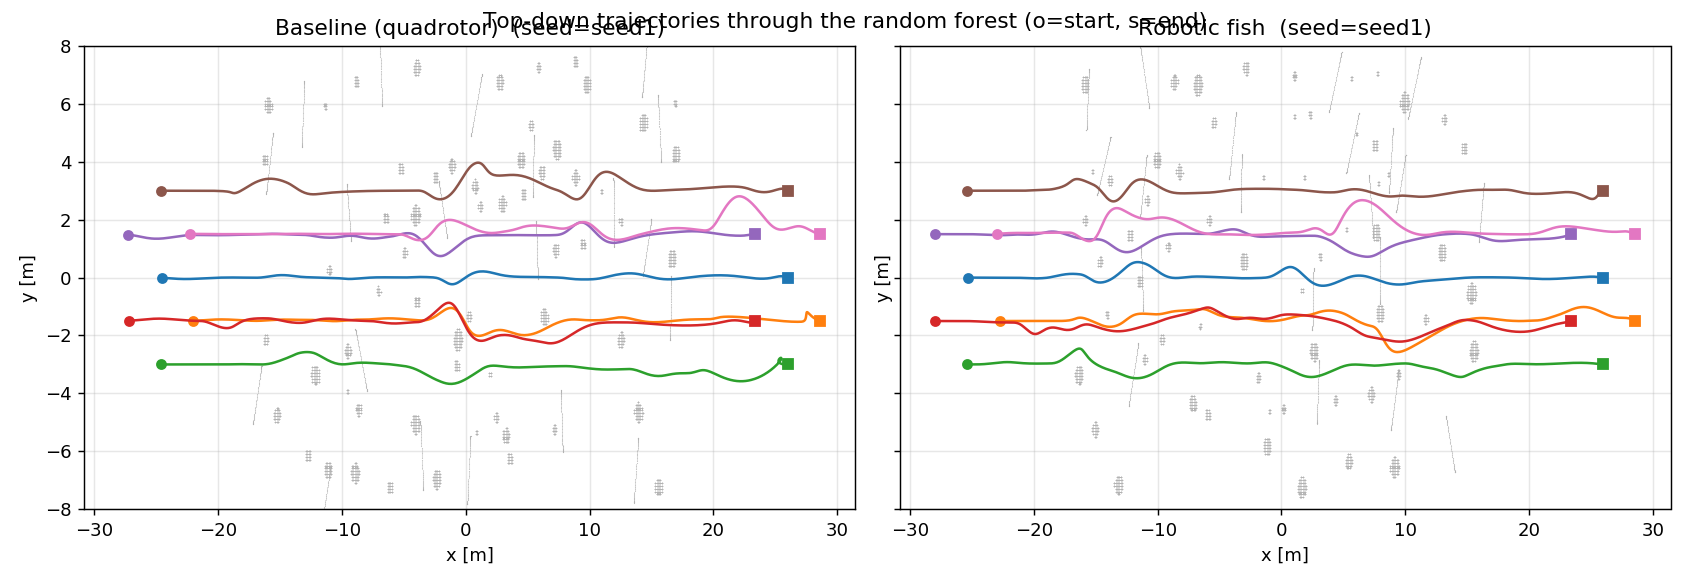
\includegraphics[width=\columnwidth]{trajectories.png}
\caption{Top-down executed paths through the random forest (seed 1), baseline
(left) versus robotic fish (right). $\bigcirc$ marks the start hexagon,
$\square$ the goal. Both conditions traverse essentially the same corridors;
path length differs by under 2\%.}
\label{fig:traj}
\end{figure}

\begin{figure}[t]
\centering
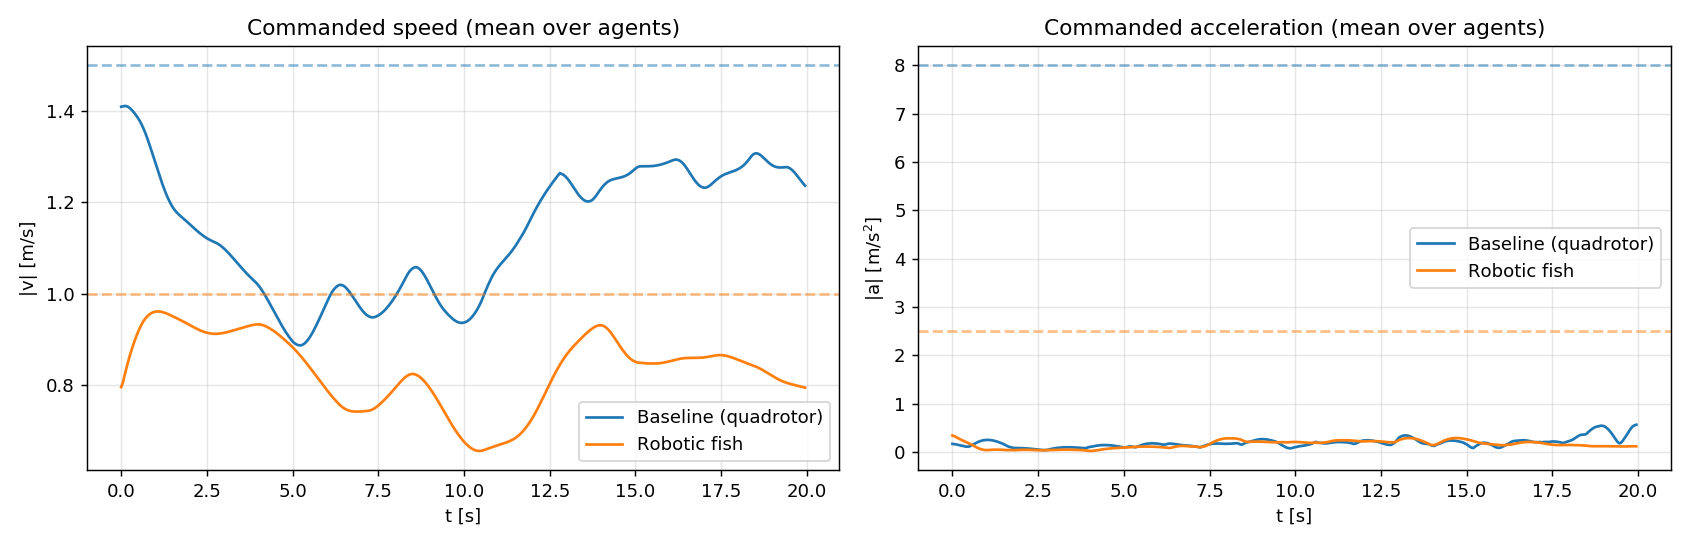
\includegraphics[width=\columnwidth]{kinematics.png}
\caption{Commanded speed (top) and acceleration (bottom), averaged over the
seven agents, for the first 20~s. Dashed lines are the per-condition
$v_{\max}$ and $a_{\max}$. The fish envelope produces lower, flatter, smoother
profiles.}
\label{fig:kin}
\end{figure}

\subsection{The Cost Is Time, Not Quality}
Because the paths are nearly identical in length ($51.4$ vs $52.3$~m, a 1.8\%
difference; Fig.~\ref{fig:traj}), the price of the gentler envelope is paid
almost entirely in time: traversal takes $\sim$44\% longer ($44.9\rightarrow
64.5$~s). Formation quality is essentially retained---mean formation RMSE
rises modestly from $0.176$ to $0.217$~m and the maximum is statistically
indistinguishable (Fig.~\ref{fig:form}). The swarm does not hold its shape
worse; it simply spends more time holding it. Fig.~\ref{fig:bars} summarizes
the trade-off across all aggregate metrics: large, well-separated kinematic
gains; a large time penalty; and formation/safety metrics that overlap within
their error bars.

\begin{figure}[t]
\centering
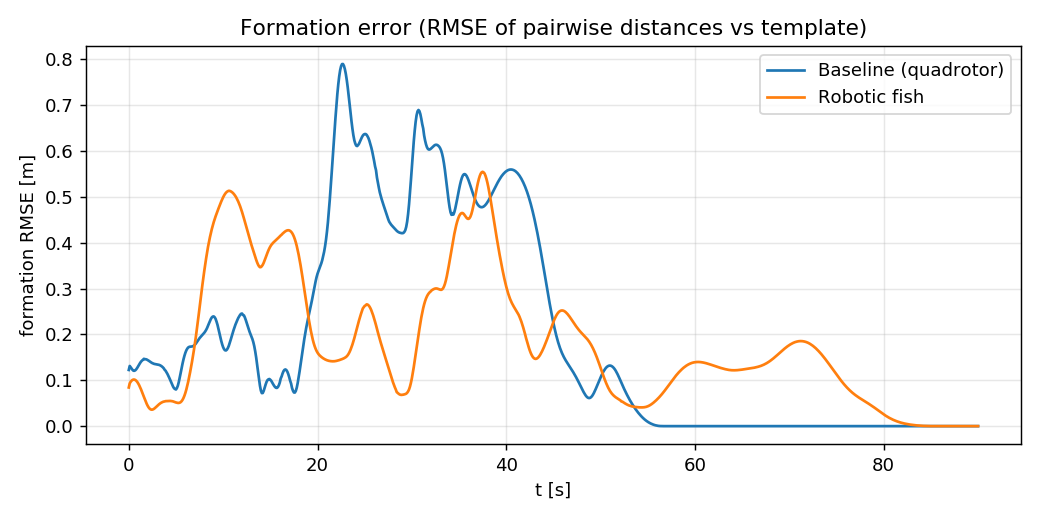
\includegraphics[width=\columnwidth]{formation.png}
\caption{Formation error (RMSE of pairwise inter-agent distances against the
hexagon template) over time. The fish trace runs slightly higher but tracks
the same envelope; the swarm holds shape in both conditions.}
\label{fig:form}
\end{figure}

\begin{figure}[t]
\centering
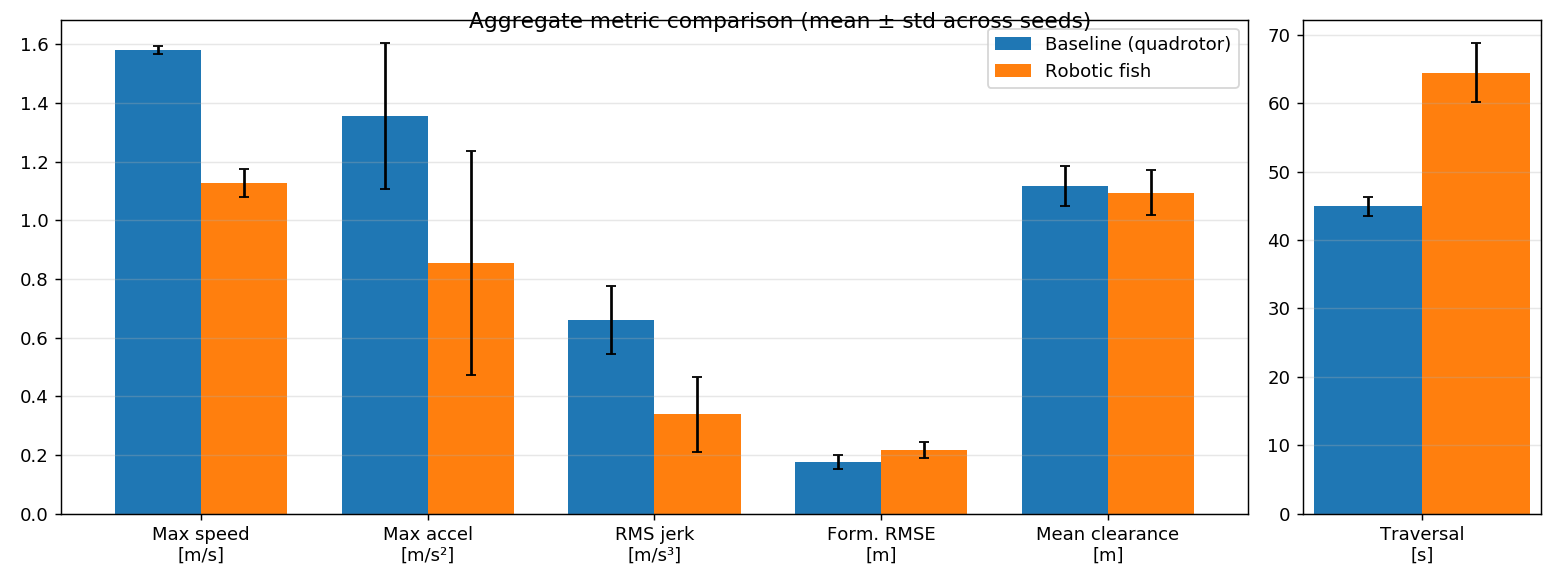
\includegraphics[width=\columnwidth]{bars.png}
\caption{Aggregate comparison (mean~$\pm$~std over five seeds) for
representative metrics. Kinematic smoothness improves substantially and
traversal time grows; formation accuracy, clearance, and safety stay within
noise.}
\label{fig:bars}
\end{figure}

\subsection{Qualitative Behavior}
Fig.~\ref{fig:rviz} shows the fish school mid-traversal and the full set of
seven executed trajectories. The hexagon is held while the school weaves
through the forest, with per-agent local occupancy clouds visible. Visually,
the school glides rather than darts---consistent with the halved jerk---yet
maintains the same spatial structure and clearance as the baseline.

\begin{figure}[t]
\centering
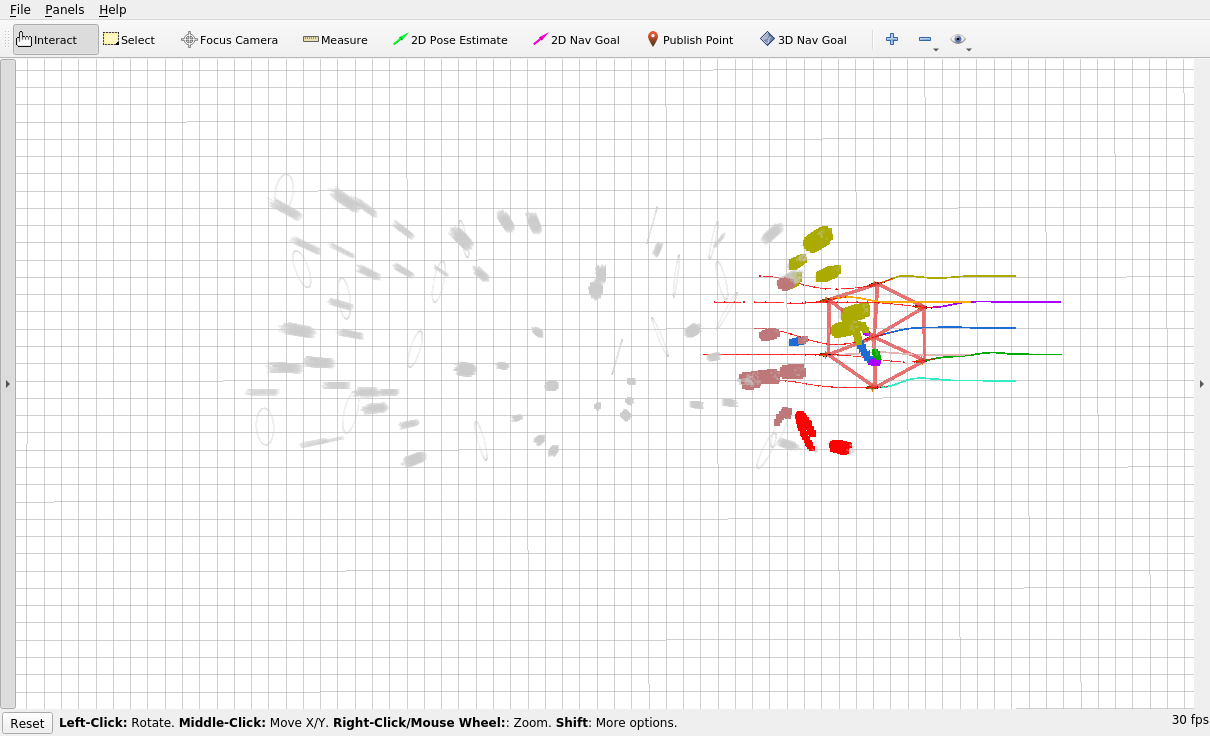
\includegraphics[width=0.49\columnwidth]{rviz_midfield.png}\hfill
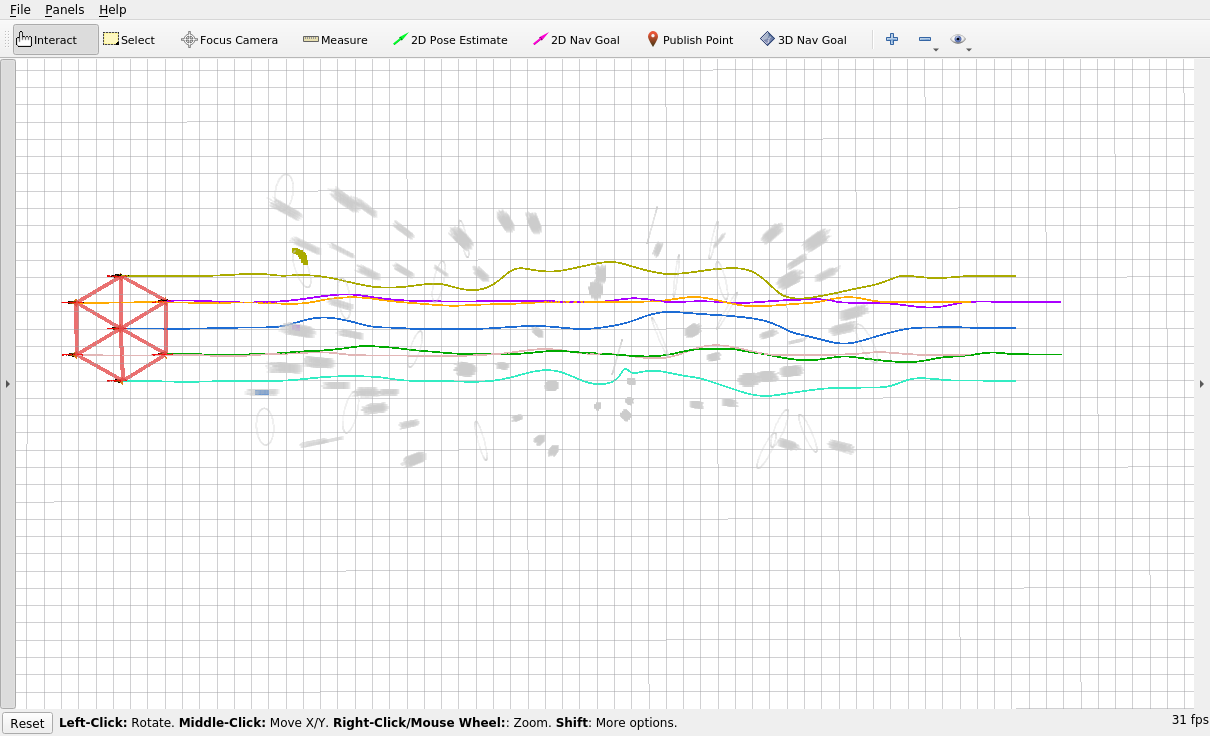
\includegraphics[width=0.49\columnwidth]{rviz_paths.png}
\caption{Qualitative views (fish condition, seed 1). Left: the seven-agent
hexagon school mid-field among the obstacle forest. Right: all seven executed
trajectories spanning the field from the start hexagon to the goal.}
\label{fig:rviz}
\end{figure}

\section{Discussion}
\label{sec:discussion}

\subsection{Interpretation}
The experiment cleanly isolates a single design knob---the dynamic-feasibility
envelope---and shows that it controls a graded, predictable trade-off:
contracting it buys substantial smoothness and slower, lower-effort motion,
and it costs time, with formation accuracy and safety essentially unchanged.
For practitioners, this means a slow, drag-limited platform can reuse a
high-performance quadrotor formation planner unchanged and obtain
school-like motion simply by tightening $\{v_{\max},a_{\max}\}$; the planner
degrades gracefully rather than failing or sacrificing formation/safety. The
fact that formation RMSE barely moves while jerk halves indicates that the
graph-similarity cost (\ref{eq:fform}) is largely decoupled from the
aggressiveness of the underlying motion---a useful robustness property.

\subsection{Scope and Limitations}
We are deliberately precise about what this study is and is not.
\emph{(i)~Fidelity.} The agents use the second-order SO(3) quadrotor model
with reduced limits, not a hydrodynamic, non-holonomic swimmer; the measured
effects therefore reflect the dynamic \emph{envelope}, not body-caudal-fin
hydrodynamics, added mass, buoyancy, or ambient currents. The fish embodiment
is a render-level re-skin. \emph{(ii)~Sample size.} Five seeds per condition
suffice to separate the large kinematic effects from their spread but render
the near-equal formation/safety metrics ``within noise,'' not proven equal; a
larger sweep with hypothesis tests would be needed to claim equivalence.
\emph{(iii)~Single environment family.} All runs use one forest density and
one start/goal geometry.

\subsection{Toward Higher Fidelity}
A natural extension replaces the SO(3) simulator and controller with a
forward-swim model: a non-holonomic constraint (bounded turn rate, motion
predominantly along the body axis), hydrodynamic drag and added-mass terms,
buoyancy, and body-caudal-fin thrust~\cite{lighthill1971large}, with an
additional non-holonomic penalty term in the trajectory optimizer. Coupling
this with implicit, vision-only coordination as demonstrated on physical fish
swarms~\cite{berlinger2021implicit} would move the study from
``school-like motion under a contracted envelope'' toward true robotic-fish
schooling, while the controlled-comparison methodology used here would carry
over directly.

\section{Conclusion}
\label{sec:conclusion}
We re-instantiated a graph-theoretic, seven-agent swarm formation planner as a
school of robotic fish by changing only the visual embodiment and the
dynamic-feasibility envelope, and quantified the consequences in a controlled,
paired simulation study over five obstacle seeds per condition. Contracting
the envelope to fish-like values roughly halves RMS jerk and cuts mean
acceleration by $\sim$44\%, yielding visibly smoother, lower-effort,
school-like motion, at a cost of $\sim$44\% longer traversal time and with
formation accuracy, inter-agent spacing, obstacle clearance, and a 100\%
success rate all preserved within run-to-run noise. The dynamic envelope is
thus a single, interpretable knob that trades time for smoothness without
compromising formation or safety, and the planner degrades gracefully under a
strongly bio-inspired regime. Future work will raise the dynamics to a true
non-holonomic, hydrodynamic swimmer and broaden the environment sweep.

\section*{Reproducibility}
The planner modifications, headless experiment harness (data collection,
metric computation, and figure generation), raw per-run logs, and all figures
in this paper are available in the project repository.

\bibliographystyle{IEEEtran}
\bibliography{refs}

\end{document}
